%
% 
%       This source code is part of
% 
%        G   R   O   M   A   C   S
% 
% GROningen MAchine for Chemical Simulations
% 
%               VERSION 2.0
% 
% Copyright (c) 1991-1999
% BIOSON Research Institute, Dept. of Biophysical Chemistry
% University of Groningen, The Netherlands
% 
% Please refer to:
% GROMACS: A message-passing parallel molecular dynamics implementation
% H.J.C. Berendsen, D. van der Spoel and R. van Drunen
% Comp. Phys. Comm. 91, 43-56 (1995)
% 
% Also check out our WWW page:
% http://md.chem.rug.nl/~gmx
% or e-mail to:
% gromacs@chem.rug.nl
% 
% And Hey:
% Gnomes, ROck Monsters And Chili Sauce
%

\chapter{Analysis}
\label{ch:analysis}
In this chapter different ways of analyzing your trajectory are described. 
The names of the corresponding analysis programs are given. 
Specific info on the in- and output of these programs can be found 
in the on-line manual at {\wwwpage}.
The output files are often produced as finished Grace/Xmgr graphs.

First in \secref{groups} the group concept in analysis is explained. 
Then the different analysis tools are presented.

%%%%%%%%%%%%%%%%%%%%%%%%%%%%%%%%%%%%%%% Groups in Analysis

\section{Groups in Analysis.}
\label{sec:groups}
{\tt make\_ndx, mk\_angndx}\\
In \chref{algorithms} it was explained how {\em groups of
atoms} can be used in the MD-program.  In most analysis programs groups
of atoms are needed to work on. Most programs can generate several default
index groups, but groups can always be read from an index file. Let's
consider a simulation of a binary mixture of components A and B. When
we want to calculate the radial distribution function (rdf)
$g_{AB}(r)$ of A with respect to B, we have to calculate
\beq
4\pi r^2 g_{AB}(r)      ~=~     V~\sum_{i \in A}^{N_A} \sum_{j \in B}^{N_B} P(r)
\eeq
where $V$ is the volume and $P(r)$ is the probability to find a B atom
at a distance $r$ from an A atom.

By having the user define the {\em atom numbers} for groups A and B in
a simple file we can calculate this $g_{AB}$ in the most general way, without
having to make any assumptions in the rdf-program about the type of 
particles. 

Groups can therefore consist of a series of {\em atom numbers}, but in
some cases also of {\em molecule numbers}.  It is also possible to
specify a series of angles by {\em triples} of {\em atom numbers},
dihedrals by {\em quadruples} of {\em atom numbers} and bonds or
vectors (in a molecule) by {\em pairs} of {\em atom numbers}. When
appropriate the type of index file will be specified for the following
analysis programs.  To help creating such \swapindex{index}{file}s ({\tt
index.ndx}), there are a couple of programs to generate them, using
either your input configuration or the topology.  To generate an
index file consisting of a series of {\em atom numbers} (as in the
example of $g_{AB}$) use {\tt \normindex{make\_ndx}}. To generate an index file
with angles or dihedrals, use {\tt \normindex{mk\_angndx}}. Of course you can also
make them by hand. The general format is presented here:

\begin{tt}
[ Oxygen ]\\
   1       4       7 \\
\end{tt}
\begin{tt}
[ Hydrogen ]\\
   2       3       5       6\\
   8       9\\
\end{tt}

First the group name is written between square brackets. The following
atom numbers may be spread out over as many lines as you like. The
atom numbering starts at 1.

\subsection{Default Groups}
\label{subsec:defaultgroups}
When no index file is supplied to analysis tools or {\tt grompp},
a number of default groups are generated to choose from:
\begin{description}
\item[{\tt System}]\mbox{}\\
        all atoms in the system
\item[{\tt Protein}]\mbox{}\\
        all protein atoms
\item[{\tt Protein-H}]\mbox{}\\
        protein atoms excluding hydrogens
\item[{\tt C-alpha}]\mbox{}\\
        C$_{\alpha}$ atoms
\item[{\tt Backbone}]\mbox{}\\
        protein backbone atoms; N, C$_{\alpha}$ and C
\item[{\tt MainChain}]\mbox{}\\
        protein main chain atoms: N, C$_{\alpha}$, C and O, including
        oxygens in C-terminus
\item[{\tt MainChain+Cb}]\mbox{}\\
        protein main chain atoms including C$_{\beta}$
\item[{\tt MainChain+H}]\mbox{}\\
        protein main chain atoms including backbone amide hydrogen and
        hydrogens on the N-terminus
\item[{\tt SideChain}]\mbox{}\\
        protein side chain atoms; that is all atoms except N,
        C$_{\alpha}$, C, O, backbone amide hydrogen, oxygens in
        C-terminus and hydrogens on the N-terminus
\item[{\tt SideChain-H}]\mbox{}\\
        protein side chain atoms excluding all hydrogens
\ifthenelse{\equal{\gmxlite}{1}}{}{
\item[{\tt Prot-Masses}]\mbox{}\\
        protein atoms excluding dummy masses (as used in virtual site
        constructions of NH$_3$ groups and Tryptophane sidechains),
        see also \secref{vsitetop}; this group is only included when
        it differs from the '{\tt Protein}' group
} % Brace matches ifthenelse test for gmxlite
\item[{\tt Non-Protein}]\mbox{}\\
        all non-protein atoms
\item[{\tt DNA}]\mbox{}\\
        all DNA atoms
\item[{\tt molecule\_name}]\mbox{}\\
        for all residues/molecules which are not recognized as protein
        or DNA, one group per residue/molecule name is generated
\item[{\tt Other}]\mbox{}\\
        all atoms which are neither protein nor DNA.
\end{description}
Empty groups will not be generated.
Most of the groups only contain protein atoms.
An atom is considered a protein atom if its residue name is listed
in the {\tt \normindex{aminoacids.dat}} file.

\subsection{Selections}
\label{subsec:selections}
{\tt g\_select}\\
{\gromacs} also includes a {\tt g\_select} tool that can be used to
select atoms based on more flexible criteria than in {\tt make\_ndx},
including selecting atoms based on their coordinates.  Currently, the
tool is experimental and only supports some basic operations, but in the
future the functionality is planned to be included in other analysis
tools as well.  Description of possible ways of selecting atoms can be
read by running {\tt g\_select} and typing {\tt help} in the selection
prompt that appears.  It is also possible to write your own analysis
tools to take advantage of the flexibility of these selections: see the
{\tt template.c} file in the {\tt share/gromacs/template} directory of
your installation for an example.

%%%%%%%%%%%%%%%%%%%%%%%%%%%%%%%%%%%%%%% Looking at your trajectory

\section{Looking at your trajectory}
\label{sec:lookwhostalking}
{\tt ngmx}\\
\begin{figure}
\centerline{
{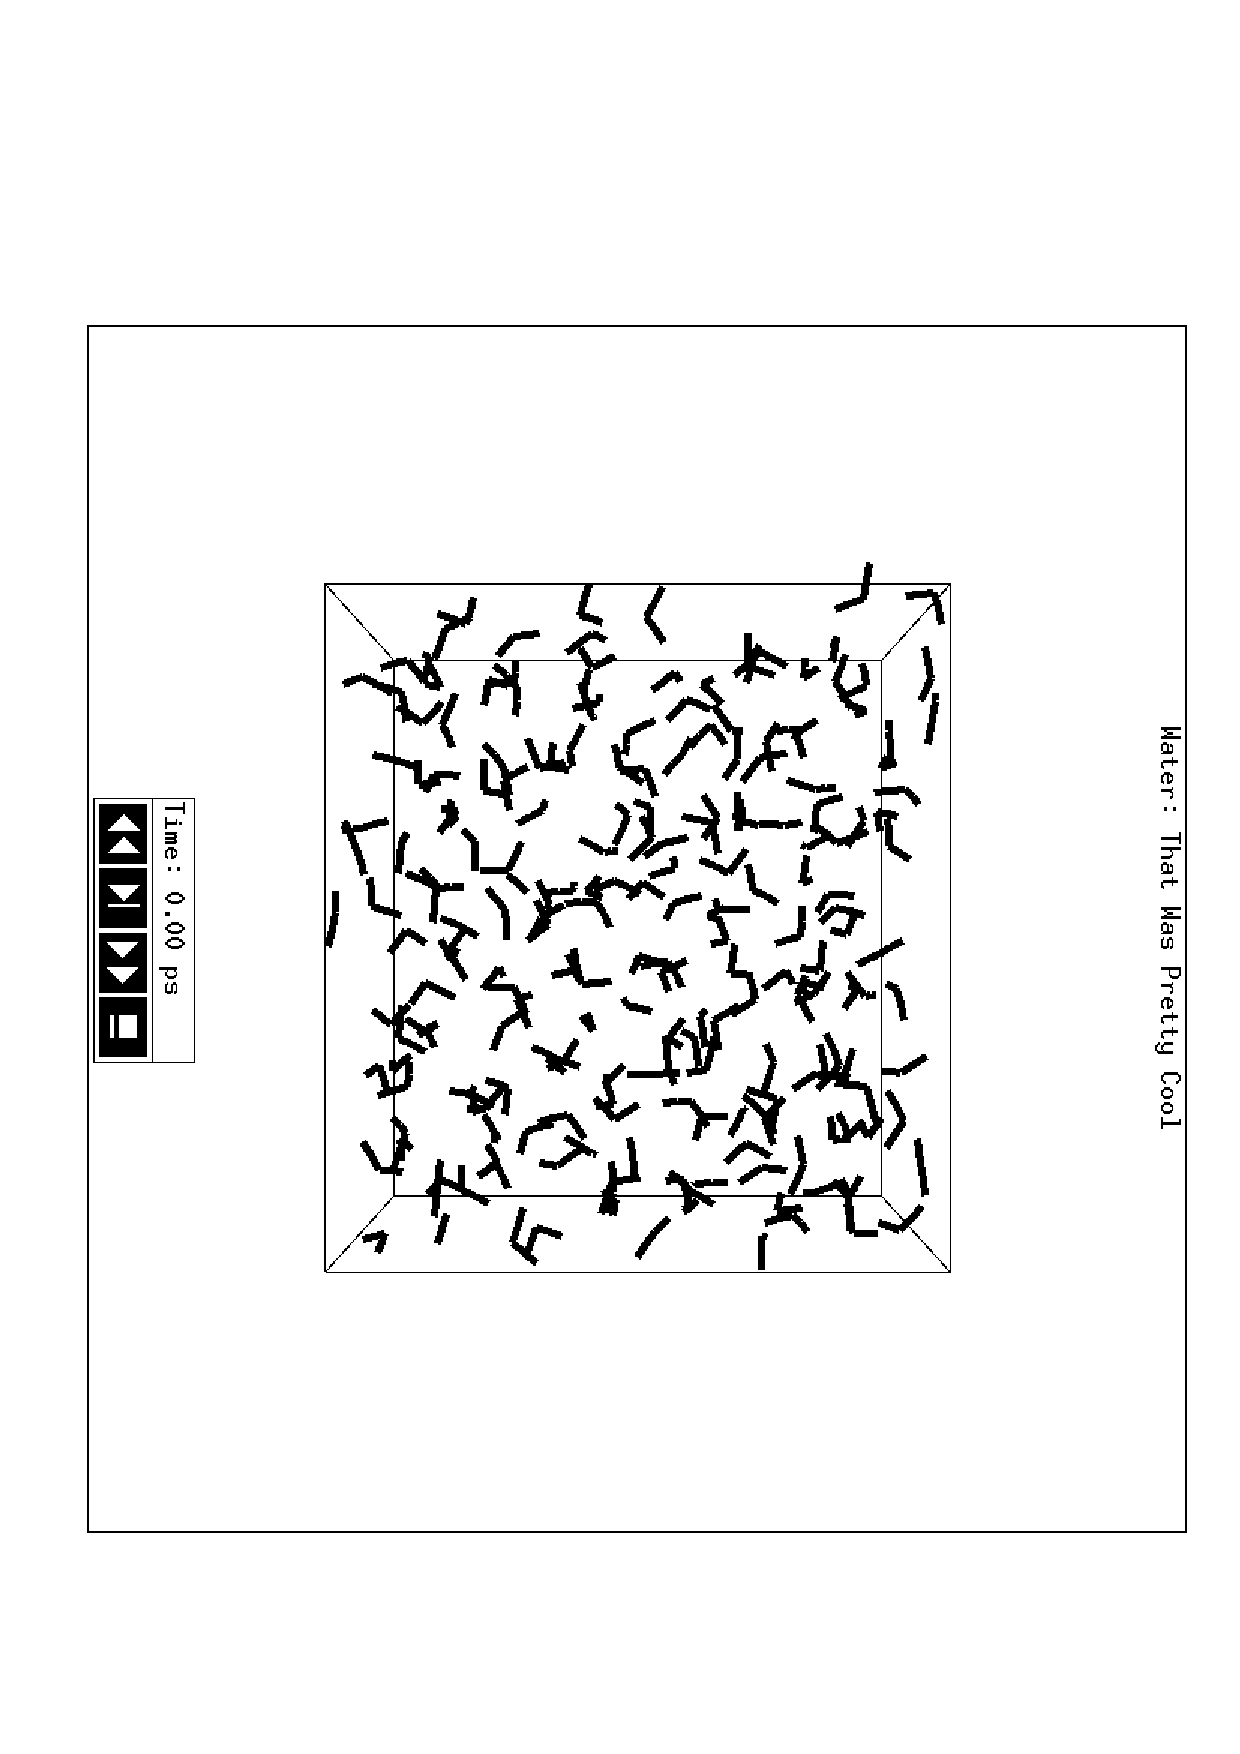
\includegraphics[width=8cm,angle=90]{plots/ngmxdump}}}
\caption{The window of {\tt ngmx} showing a box of water.}
\label{fig:ngmxdump}
\end{figure}

Before analyzing your trajectory it is often informative to look at
your trajectory first. Gromacs comes with a simple trajectory
viewer {\tt \normindex{ngmx}}; the advantage with this one is that it does not
require OpenGL, which usually isn't present e.g. on supercomputers.
It is also possible to generate a
hard-copy in Encapsulated Postscript format, see
\figref{ngmxdump}. If you want a faster and more fancy viewer
 there are several programs
that can read the {\gromacs} trajectory formats -- have a look at our
homepage {\wwwpage} for updated links. 

%%%%%%%%%%%%%%%%%%%%%%%%%%%%%%%%%%%%%%% General properties

\section{General properties}
\label{sec:genprop}
{\tt g\_energy, g\_traj}\\
To analyze some or all {\em energies} and other properties, such as
{\em total pressure}, {\em pressure tensor}, {\em density}, {\em
box-volume} and {\em box-sizes}, use the program {\tt \normindex{g\_energy}}.  A
choice can be made from a list a set of energies, like potential,
kinetic or total energy, or individual contributions, like
Lennard-Jones or dihedral energies.

The {\em center-of-mass velocity}, defined as
\beq
{\bf v}_{com} = {1 \over M} \sum_{i=1}^N m_i {\bf v}_i
\eeq
with $M = \sum_{i=1}^N m_i$ the total mass of the system, can be
monitored in time by the program {\tt \normindex{g\_com}}. It is however
recommended to remove the center-of-mass velocity every step (see
\chref{algorithms})!

%%%%%%%%%%%%%%%%%%%%%%%%%%%%%%%%%%%%%%% Radial distribution functions 

\section{Radial distribution functions}
\label{sec:rdf}
{\tt g\_rdf}\\
The {\em radial distribution function} (rdf) or pair correlation
function $g_{AB}(r)$ between particles of type $A$ and $B$ is defined
in the following way:
\newcommand{\dfrac}[2]{\displaystyle \frac{#1}{#2}}
\beq
\begin{array}{rcl}
g_{AB}(r)&=&    \dfrac{\langle \rho_B(r) \rangle}{\langle\rho_B\rangle_{local}}         \\
         &=&    \dfrac{1}{\langle\rho_B\rangle_{local}}\dfrac{1}{N_A}
                \sum_{i \in A}^{N_A} \sum_{j \in B}^{N_B} 
                \dfrac{\delta( r_{ij} - r )}{4 \pi r^2}         \\
\end{array}
\eeq
with $\langle\rho_B(r)\rangle$ the particle density of type $B$ at a distance $r$
around particles $A$, and $\langle\rho_B\rangle_{local}$ the particle density of
type $B$ averaged over all spheres around particles $A$ with radius
$r_{max}$ (see \figref{rdfex}C).

\begin{figure}
\centerline{
{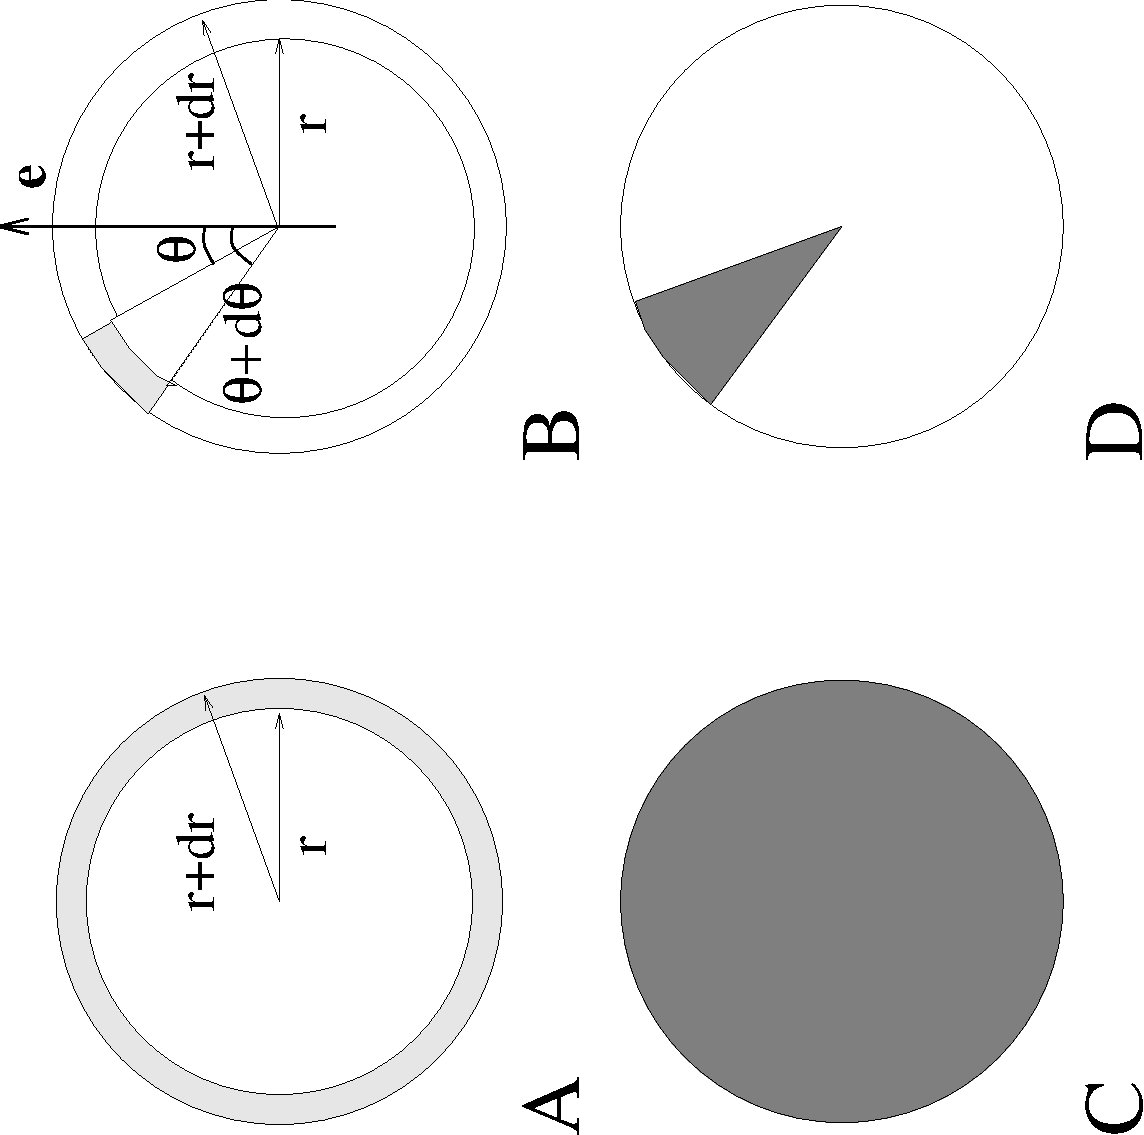
\includegraphics[width=7cm,angle=270]{plots/rdf}}}
\caption[Definition of slices in {\tt g\_rdf}.]{Definition of slices
in {\tt g\_rdf}: A. $g_{AB}(r)$. B. $g_{AB}(r,\theta)$. The slices are
colored grey. C. Normalization $\langle\rho_B\rangle_{local}$. D. Normalization
$\langle\rho_B\rangle_{local,\:\theta }$. Normalization volumes are colored grey.}
\label{fig:rdfex}
\end{figure}

Usually the value of $r_{max}$ is half of the box length.  The
averaging is also performed in time.  In practice the analysis program
{\tt \normindex{g\_rdf}} divides the system into spherical slices (from $r$ to
$r+dr$, see \figref{rdfex}A) and makes a histogram in stead of
the $\delta$-function. An example of the rdf of Oxygen-Oxygen in
SPC-water~\cite{Berendsen81} is given in \figref{rdf}.

\begin{figure}
\centerline{
{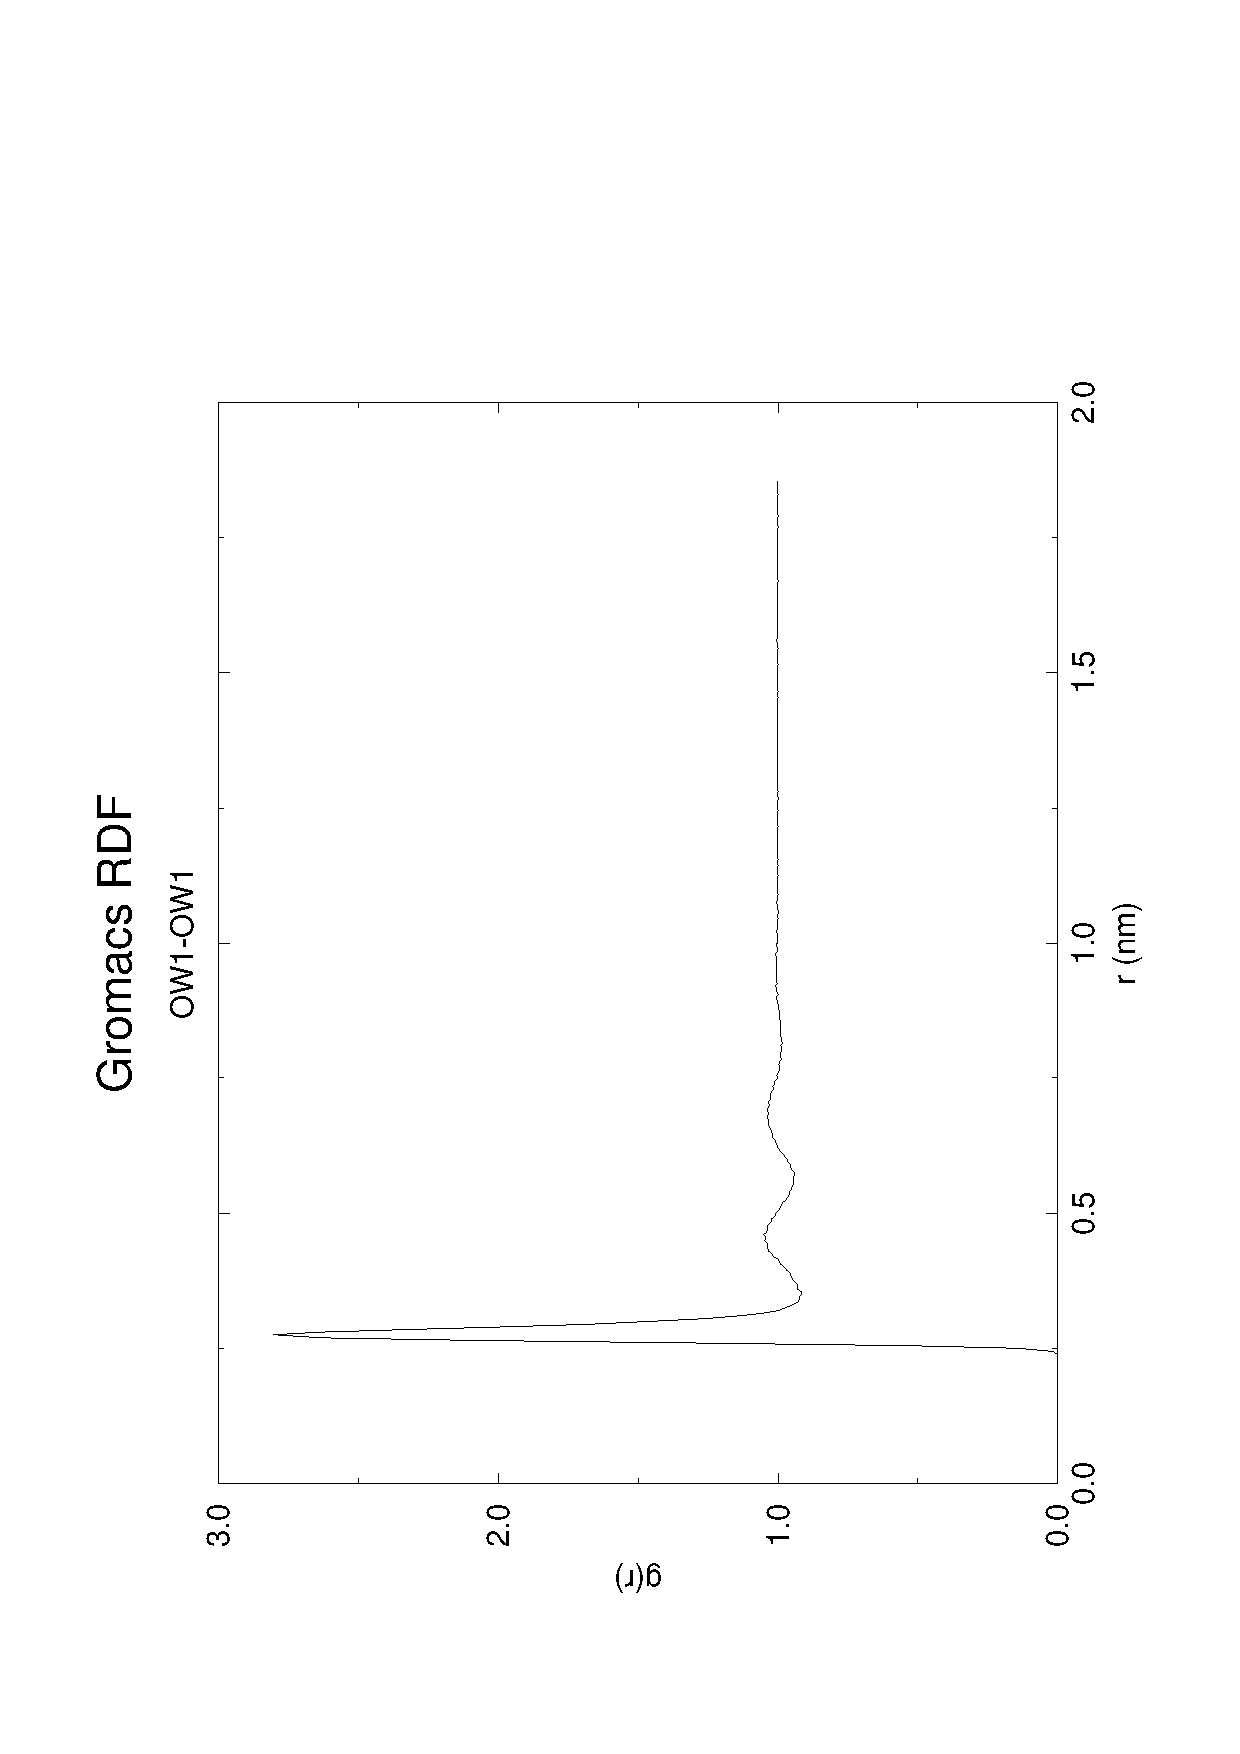
\includegraphics[width=8cm]{plots/rdfO_O}}}
\caption{$g_{OO}(r)$ for Oxygen-Oxygen of SPC-water.}
\label{fig:rdf}
\end{figure}

With {\tt g\_rdf} it is also possible to calculate an angle dependent rdf 
$g_{AB}(r,\theta)$, where the angle $\theta$ is defined with respect to a 
certain laboratory axis ${\bf e}$, see \figref{rdfex}B.
\bea 
g_{AB}(r,\theta) &=& {1 \over \langle\rho_B\rangle_{local,\:\theta }} {1 \over N_A} \sum_{i \in A}^{N_A} \sum_{j \in B}^{N_B} {\delta( r_{ij} - r ) \delta(\theta_{ij} -\theta) \over 2 \pi r^2 sin(\theta)}\\
cos(\theta_{ij}) &=& {{\bf r}_{ij} \cdot {\bf e} \over \|r_{ij}\| \;\| e\| }
\eea
This $g_{AB}(r,\theta)$ is useful for analyzing anisotropic systems. 
Note that in this case the normalization $\langle\rho_B\rangle_{local,\:\theta}$ is 
the average density in all angle slices from $\theta$ to $\theta + d\theta$ 
up to $r_{max}$, so angle dependent, see \figref{rdfex}D.

%%%%%%%%%%%%%%%%%%%%%%%%%%%%%%%%%%%%%%% Correlation functions 
\ifthenelse{\equal{\gmxlite}{1}}{}{

\section{Correlation functions}
\label{sec:corr}

\subsection{Theory of correlation functions}
The theory of correlation functions is well established~\cite{Allen87}.
However we want to describe here the implementation of the various 
\normindex{correlation} function flavors in the {\gromacs} code.
The definition of the \swapindex{autocorrelation}{function} (ACF)
$C_f(t)$ for a property $f(t)$ is
\beq
C_f(t)  ~=~     \left\langle f(\xi) f(\xi+t)\right\rangle_{\xi}
\label{eqn:corr}
\eeq
where the notation on the right hand side means averaging over $\xi$, {\ie} over
time origins.
It is also possible to compute cross-correlation function from two properties
$f(t)$ and $g(t)$:
\beq
C_{fg}(t) ~=~   \left\langle f(\xi) g(\xi+t)\right\rangle_{\xi}
\eeq
however, in {\gromacs} there is no standard mechanism to do this
({\bf note:} you can use the {\tt \normindex{xmgr}} program to compute cross correlations).
The integral of the correlation function over time is the 
correlation time $\tau_f$:
\beq
\tau_f  ~=~     \int_0^{\infty} C_f(t) {\rm d} t
\label{eqn:corrtime}
\eeq

In practice correlation functions are calculated based on data points with
discrete time intervals {$\Delta$t}, so that the ACF from an MD simulation is:
\beq
C_f(j\Delta t)  ~=~     \frac{1}{N-j}\sum_{i=0}^{N-1-j} f(i\Delta t) f((i+j)\Delta t)
\label{eqn:corrmd}
\eeq
where $N$ is the number of available time frames for the calculation.
The resulting ACF is
obviously only available at time points with the same interval {$\Delta$t}.
Since for many applications it is necessary to know  the short time behavior
of the ACF ({\eg} the first 10 ps) this often means that we have to save the
atomic coordinates with short intervals.
Another implication of \eqnref{corrmd} is that in principle we can not compute
all points of the ACF with the same accuracy, since we have $N-1$ data points
for $C_f(\Delta t)$ but only 1 for $C_f((N-1)\Delta t)$. However, if we decide to
compute only an ACF of length $M\Delta t$, where $M \leq N/2$ we can compute 
all points with the same statistical accuracy:
\beq
C_f(j\Delta t)  ~=~ \frac{1}{M}\sum_{i=0}^{N-1-M} f(i\Delta t)f((i+j)\Delta t)
\eeq
here of course $j < M$.
$M$ is sometimes referred to as the \normindex{time lag} of the correlation function. 
When we decide to do this, we intentionally do not use all the available points
for very short time intervals ($j << M$), but it makes it easier to interpret
the results.
Another aspect that may not be neglected when computing
ACFs from simulation, is that usually the time origins $\xi$ (\eqnref{corr})
are not statistically independent, which may introduce a bias in the results.
This can be tested using a block-averaging procedure, where only time origins
with a spacing at least the length of the time lag are included, {\eg} using 
$k$ time origins with spacing of $M\Delta t$ (where $kM \leq N$):
\beq
C_f(j\Delta t)  ~=~ \frac{1}{k}\sum_{i=0}^{k-1} f(iM\Delta t)f((iM+j)\Delta t)
\eeq
However, one
needs very long simulations to get good accuracy this way, because there are 
many fewer points that contribute to the ACF.

\subsection{Using FFT for computation of the ACF}
The computational cost for calculating an ACF according to \eqnref{corrmd}
is proportional to $N^2$, which is considerable. However, this can be improved
by using fast Fourier transforms to do the convolution~\cite{Allen87}.

\subsection{Special forms of the ACF}
There are some important varieties on the ACF, {\eg} the ACF of a vector \ve{p}:
\beq
C_{\ve{p}}(t) ~=~       \int_0^{\infty} P_n(\cos\angle\left(\ve{p}(\xi),\ve{p}(\xi+t)\right) {\rm d} \xi
\label{eqn:corrleg}
\eeq
where $P_n(x)$ is the $n^{th}$ order Legendre polynomial
\footnote{$P_0(x) = 1$, $P_1(x) = x$, $P_2(x) = (3x^2-1)/2$}.
Such correlation times 
can actually be obtained experimentally using {\eg} NMR or other relaxation 
experiments. {\gromacs} can compute correlations using 
the 1${st}$ and 2$^{nd}$ order Legendre polynomial (\eqnref{corrleg}).
This can a.o. be used for rotational autocorrelation ({\tt \normindex{g\_rotacf}}), 
dipole autocorrelation ({\tt \normindex{g\_dipoles}}).

In order to study torsion angle dynamics we define a dihedral 
autocorrelation function as~\cite{Spoel97a}:
\beq
C(t)    ~=~     \left\langle \cos(\theta(\tau)-\theta(\tau+t))\right\rangle_{\tau}
\label{eqn:coenk}
\eeq
Note that this is not a  product of two functions 
as is generally used for correlation
functions, but it may be rewritten as the sum of two products:
\beq
C(t)    ~=~     \left\langle\cos(\theta(\tau))\cos(\theta(\tau+t))\,+\,\sin(\theta(\tau))\sin(\theta(\tau+t))\right\rangle_{\tau}
\label{eqn:cot}
\eeq

\subsection{Some Applications}
The program {\tt \normindex{g\_velacc}} calculates this {\em Velocity Auto Correlation 
Function}.
\beq
C_{\ve{v}} (\tau) ~=~ \langle {\ve{v}}_i(\tau) \cdot {\ve{v}}_i(0) \rangle_{i \in A}
\eeq
The self diffusion coefficient can be calculated using the Green-Kubo 
relation~\cite{Allen87}
\beq
D_A ~=~ {1\over 3} \int_0^{\infty} \langle {\bf v}_i(t) \cdot {\bf v}_i(0) \rangle_{i \in A} \; dt
\eeq
which is just the integral of the velocity autocorrelation function.
There is a widely held belief that the velocity ACF converges faster than the mean
square displacement (\secref{msd}), which can also be used for the computation of 
diffusion constants. However, Allen \& Tildesly~\cite{Allen87} 
warn us that the long time 
contribution to the velocity ACF can not be ignored, so care must be taken.

Another important quantity is the dipole correlation time. The {\em dipole 
correlation function} for particles $A$ is calculated as follows by 
{\tt \normindex{g\_dipoles}}:
\beq
C_{\mu} (\tau) ~=~
\langle {\bf \mu}_i(\tau) \cdot {\bf \mu}_i(0) \rangle_{i \in A}
\eeq
with ${\bf \mu}_i = \sum_{j \in i} {\bf r}_j q_j$. The dipole correlation time 
can be computed using \eqnref{corrtime}.
For some applications see~\cite{Spoel98a}.

The \normindex{viscosity} of a liquid can be related to the correlation 
time of the Pressure tensor $\ve{P}$~\cite{PSmith93c,Balasubramanian96}.
{\tt \normindex{g\_energy}} can compute the viscosity,
but this is not very accurate~\cite{Hess2002a}
(actually the values do not converge...).
} % Brace matches ifthenelse test for gmxlite

\section{Mean Square Displacement}
\label{sec:msd}
{\tt g\_msd}\\
To determine the self \swapindex{diffusion}{coefficient} $D_A$ of
particles $A$ one can use the \normindex{Einstein
relation}~\cite{Allen87} \
\beq 
\lim_{t \rightarrow \infty} \langle
\|{\bf r}_i(t) - {\bf r}_i(0)\|^2 \rangle_{i \in A} ~=~ 6 D_A t 
\eeq
This {\em Mean Square Displacement} and $D_A$ are calculated by the
program {\tt \normindex{g\_msd}}. Normally an index file containing
atom numbers is used and the MSD is averaged over atoms.  For
molecules consisting of more than one atom, ${\bf r}_i$ can be taken
as the center of mass positions of the molecules. In that case you
should use an index file with molecule numbers. The results will be
nearly identical to averaging over atoms, however. The {\tt g\_msd}
program can
also be used for calculating diffusion in one or two dimensions. This
is useful for studying lateral diffusion on interfaces.

An example of the mean square displacement of SPC-water is given in
\figref{msdwater}.

\begin{figure}
\centerline{
{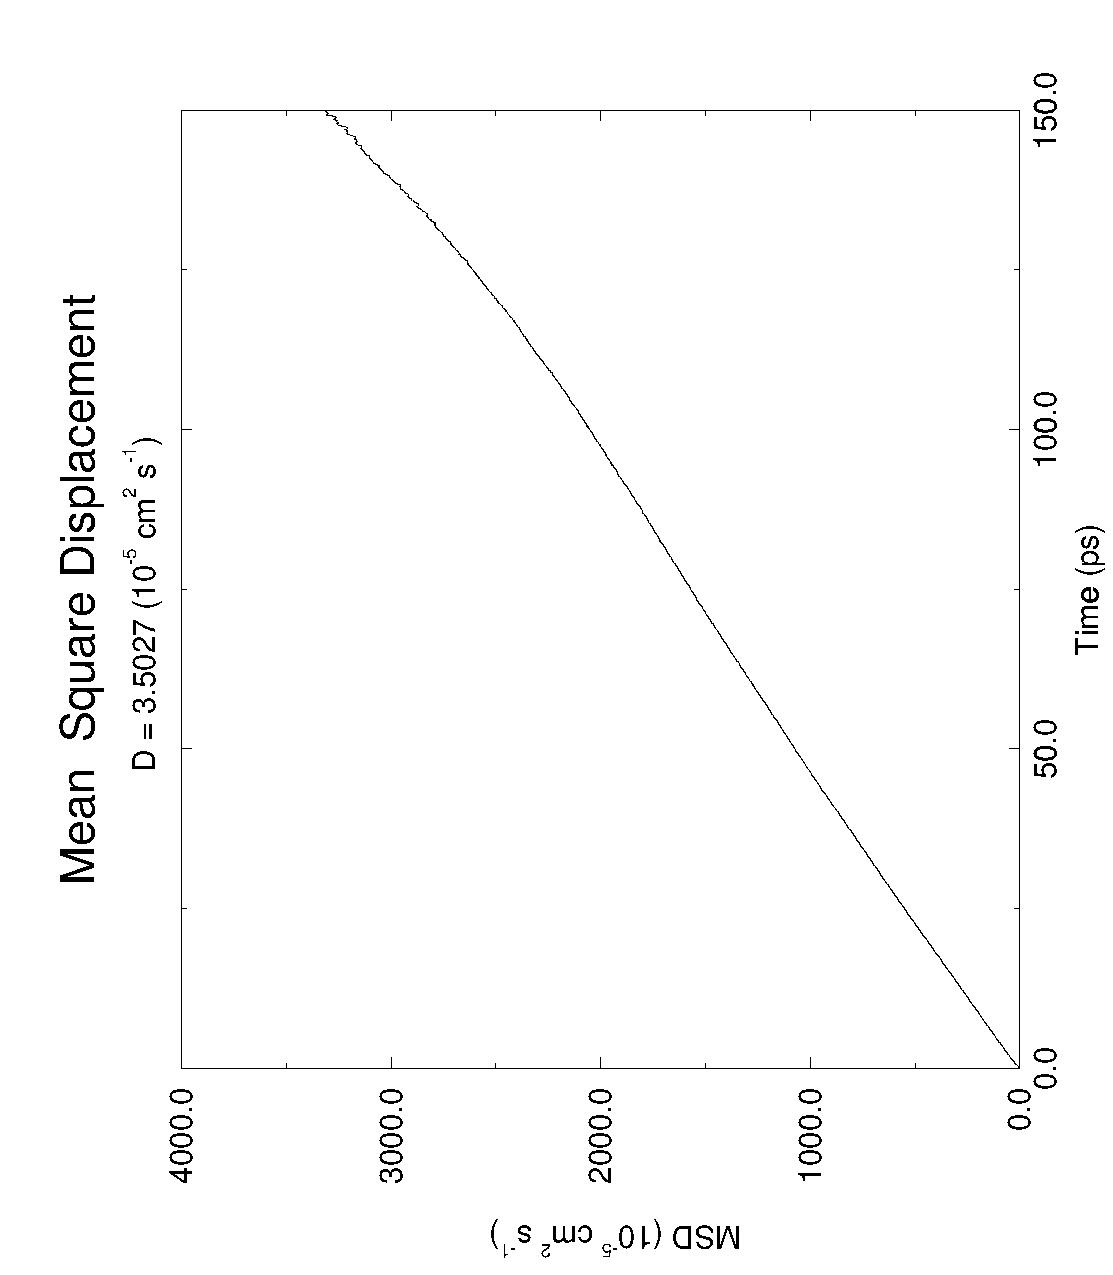
\includegraphics[width=8cm]{plots/msdwater}}}
\caption{Mean Square Displacement of SPC-water.}
\label{fig:msdwater}
\end{figure}

\ifthenelse{\equal{\gmxlite}{1}}{}{
% 
%%%%%%%%%%%%%%%%%%%%% Bonds, angles and dihedral %%%%%%%%%%%%%%%%%%%
% 
\section{Bonds, angles and dihedrals}
\label{sec:bad}
{\tt g\_bond, g\_angle, g\_sgangle}\\
To monitor specific {\em bonds} in your molecules during time, the program 
{\tt \normindex{g\_bond}} calculates the distribution of the bond length in time. 
The index file consists of pairs of atom numbers, for example\\

\begin{tt}
[ bonds\_1 ]\\
 1     2\\
 3     4\\
 9    10\\
\end{tt}
\begin{tt}
[ bonds\_2 ]\\
12    13\\
\end{tt}

The program {\tt \normindex{g\_angle}} calculates the distribution of {\em angles} and 
{\em dihedrals} in time. It also gives the average angle or dihedral. 
The index file consists of triplets or quadruples of atom numbers:

\begin{tt}
[ angles ]\\
 1     2     3\\
 2     3     4\\
 3     4     5\\
\end{tt}
\begin{tt}
[ dihedrals ]\\
 1     2     3     4\\
 2     3     5     5\\
\end{tt}

For the dihedral angles you can use either the ``biochemical convention'' 
($\phi = 0 \equiv cis$) or ``polymer convention'' ($\phi = 0 \equiv trans$), 
see \figref{dih_def}.

\begin{figure}
\centerline{
{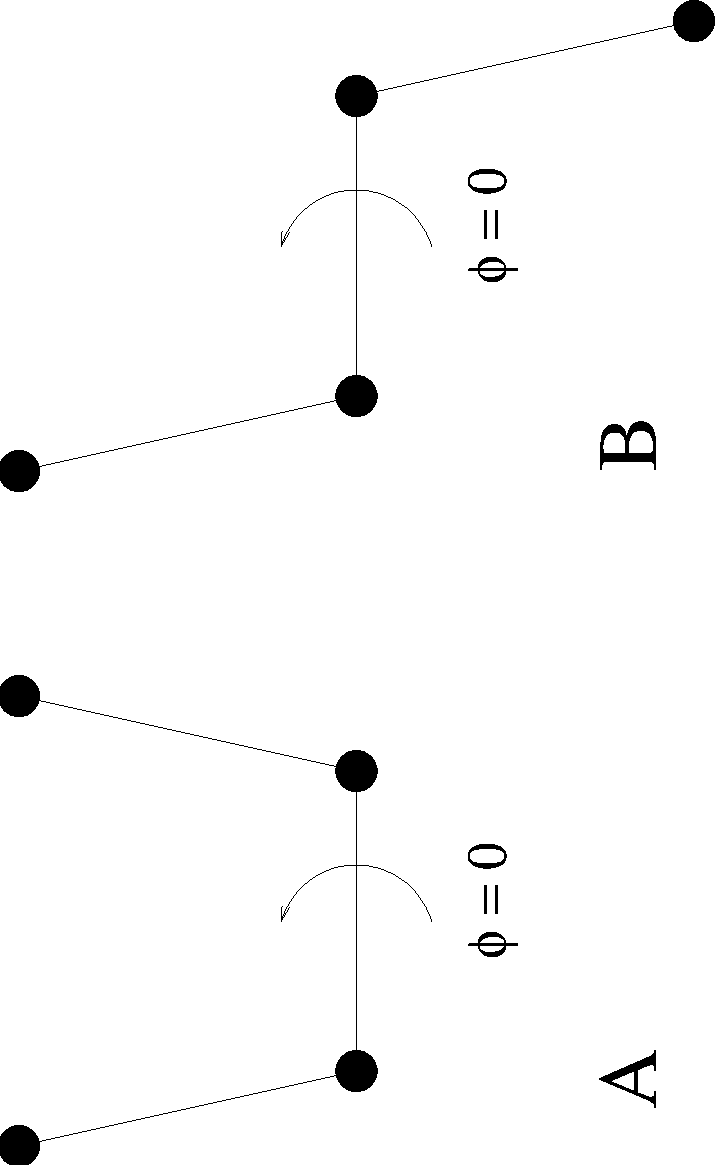
\includegraphics[width=3.5cm,angle=270]{plots/dih_def}}}
\caption[Dihedral conventions.]{Dihedral conventions: A. ``Biochemical
convention''. B. ``Polymer convention''.}
\label{fig:dih_def}
\end{figure}

To follow specific {\em angles} in time between two vectors, a vector
and a plane or two planes (defined by 2, resp. 3 atoms inside your
molecule, see \figref{sgangle}A, B, C), use the program {\tt
\normindex{g\_sgangle}}.

\begin{figure}
\centerline{
{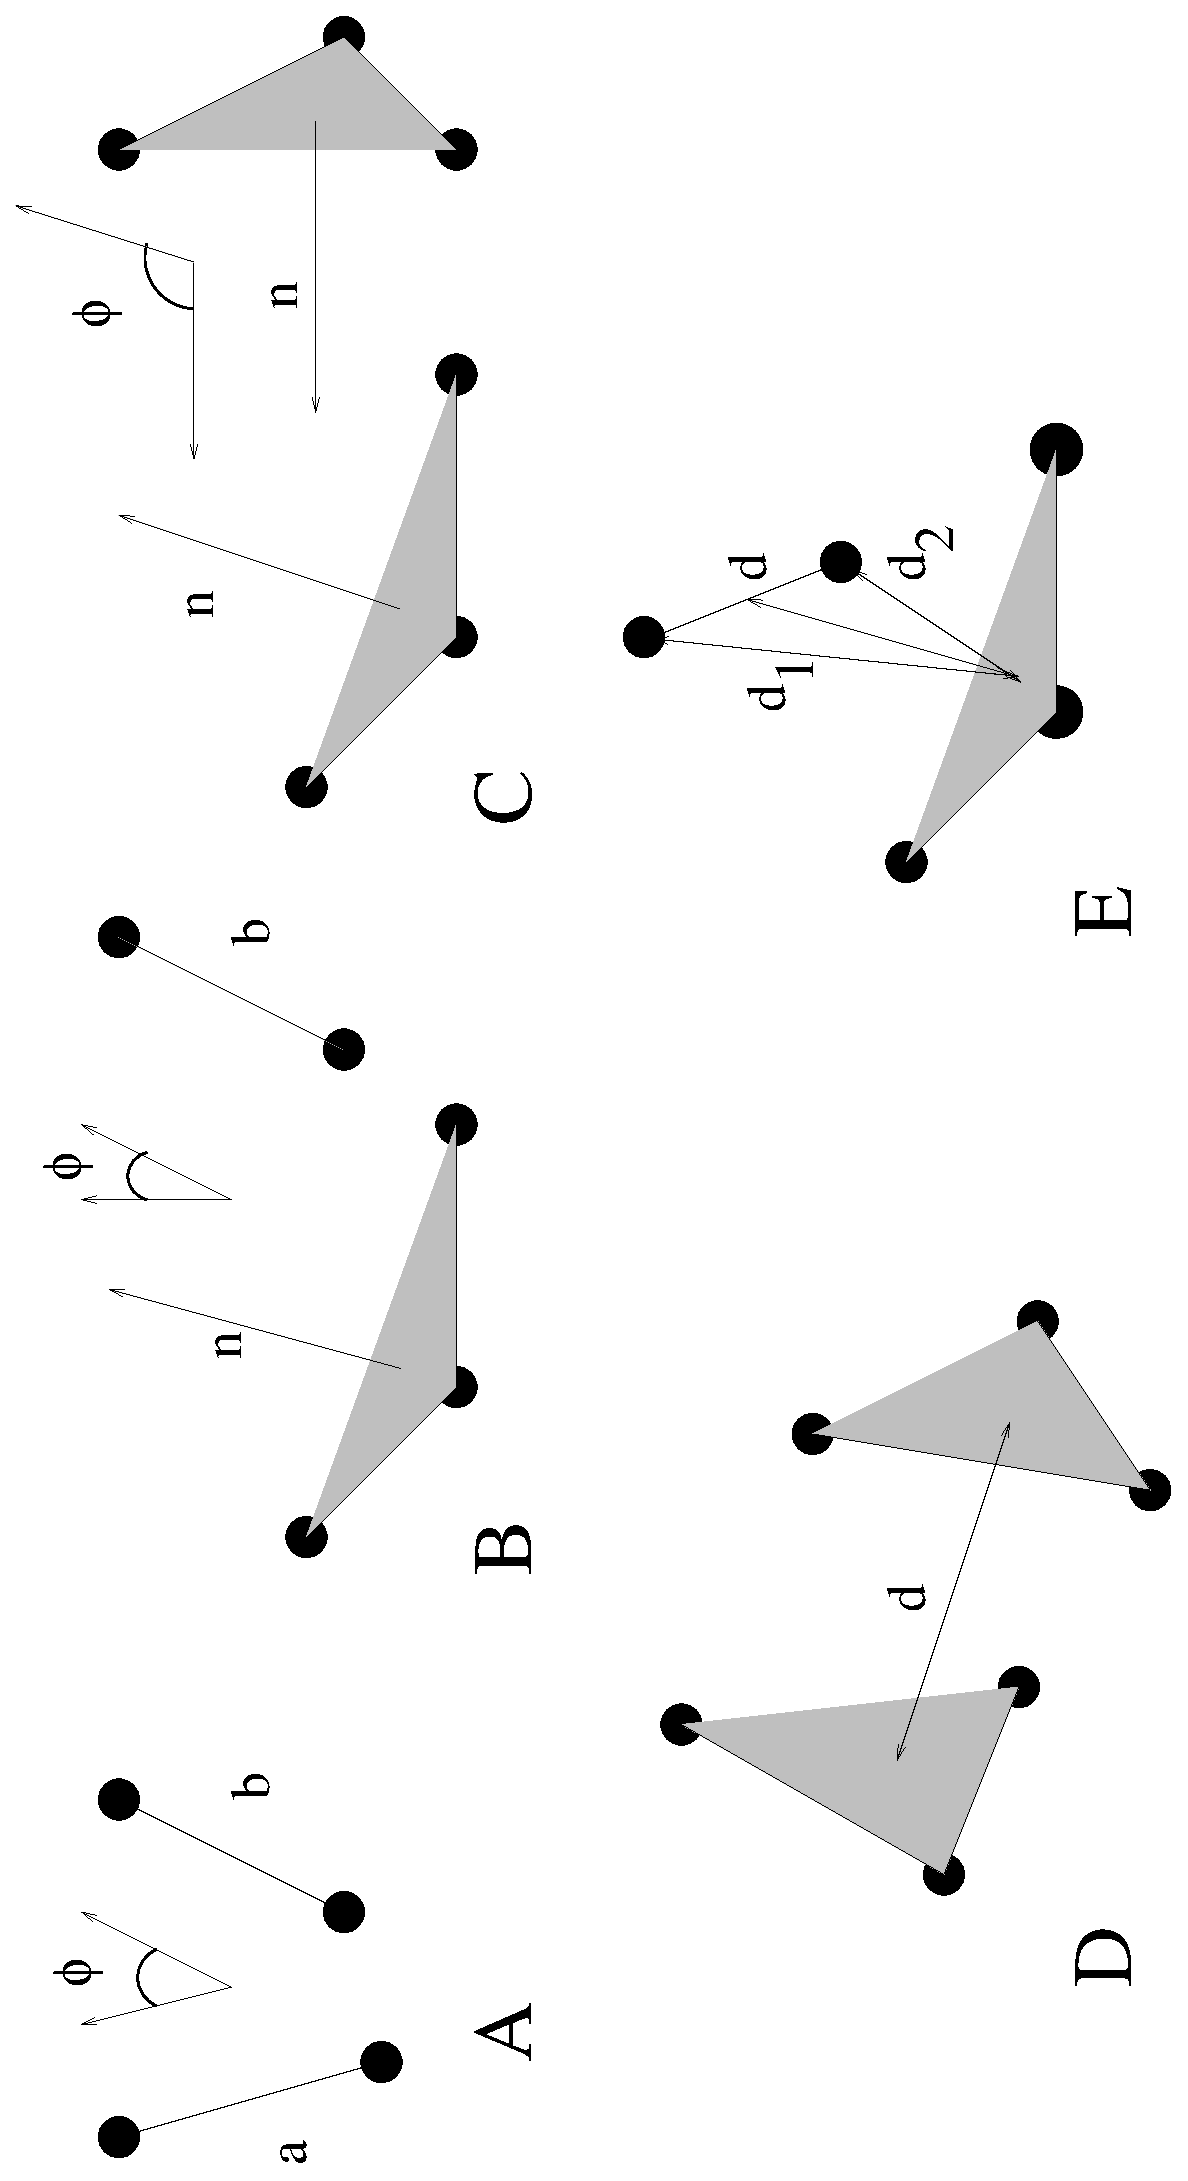
\includegraphics[width=6.5cm,angle=270]{plots/sgangle}}}
\caption[Options of {\tt g\_sgangle}.]{Options of {\tt g\_sgangle}: A. Angle between 2 vectors. B. Angle between a vector and the normal of a plane. C. Angle between two planes. D. Distance between the geometrical centers of 2 planes. E. Distances between a vector and the center of a plane.}
\label{fig:sgangle}
\end{figure}

For planes it uses the normal vector perpendicular to the plane.  It
can also calculate the {\em distance} $d$ between the geometrical
center of two planes (see \figref{sgangle}D), and the distances
$d_1$ and $d_2$ between 2 atoms (of a vector) and the center of a
plane defined by 3 atoms (see \figref{sgangle}D). It further
calculates the distance $d$ between the center of the plane and the
middle of this vector.  Depending on the input groups ({\ie} groups of
2 or 3 atom numbers), the program decides what angles and distances to
calculate. For example, the index-file could look like this:

\begin{tt}
[ a\_plane ]\\
 1     2     3\\
\end{tt}
\begin{tt}
[ a\_vector ]\\
 3     4     5\\
\end{tt}
} % Brace matches ifthenelse test for gmxlite

%%%%%%%%%%%%%%%%%%%%%%%%%%%%%%%%%%%%%%% Radius of gyration and distances

\section{Radius of gyration and distances}
\label{sec:rg}
{\tt g\_gyrate, g\_sgangle, g\_mindist, g\_mdmat, xpm2ps}\\
To have a rough measure for the compactness of a structure, you can calculate 
the {\em radius of gyration} with the program {\tt \normindex{g\_gyrate}} as follows:
\beq
R_g ~=~ \left({\frac{\sum_i \|{\bf r}_i\|^2 m_i}{\sum_i m_i}}\right)^{\half}
\label{eqn:rg}
\eeq
where $m_i$ is the mass of atom $i$ and ${\bf r}_i$ the position of 
atom $i$ with respect to the center of mass of the molecule. It is especially 
useful to characterize polymer solutions and proteins.

Sometimes it is interesting to plot the {\em distance} between two atoms,
or the {\em minimum} distance between two groups of atoms
({\eg}: protein side-chains in a salt bridge). 
To calculate these distances between certain groups there are several 
possibilities:
\begin{description}
\item[$\bullet$] 
The {\em distance between the geometrical centers} of two groups can be 
calculated with the program {\tt \normindex{g\_sgangle}}, as explained in \secref{bad}. 
\item[$\bullet$] 
The {\em minimum distance} between two groups of atoms during time 
can be calculated with the program {\tt \normindex{g\_mindist}}. It also calculates the 
{\em number of contacts} between these groups 
within a certain radius $r_{max}$.
\item[$\bullet$] 
To monitor the {\em minimum distances between amino-acid residues} 
within a (protein) molecule, you can use 
the program {\tt \normindex{g\_mdmat}}. This minimum distance between two residues
A$_i$ and A$_j$ is defined as the smallest distance between any pair of 
atoms (i $\in$ A$_i$, j $\in$ A$_j$).
The output is a symmetrical matrix of smallest distances 
between all residues.
To visualize this matrix, you can use a program such as {\tt xv}.
If you want to view the axes and legend or if you want to print
the matrix, you can convert it with 
{\tt xpm2ps} into a Postscript picture, see \figref{mdmat}.
\begin{figure}
\centerline{
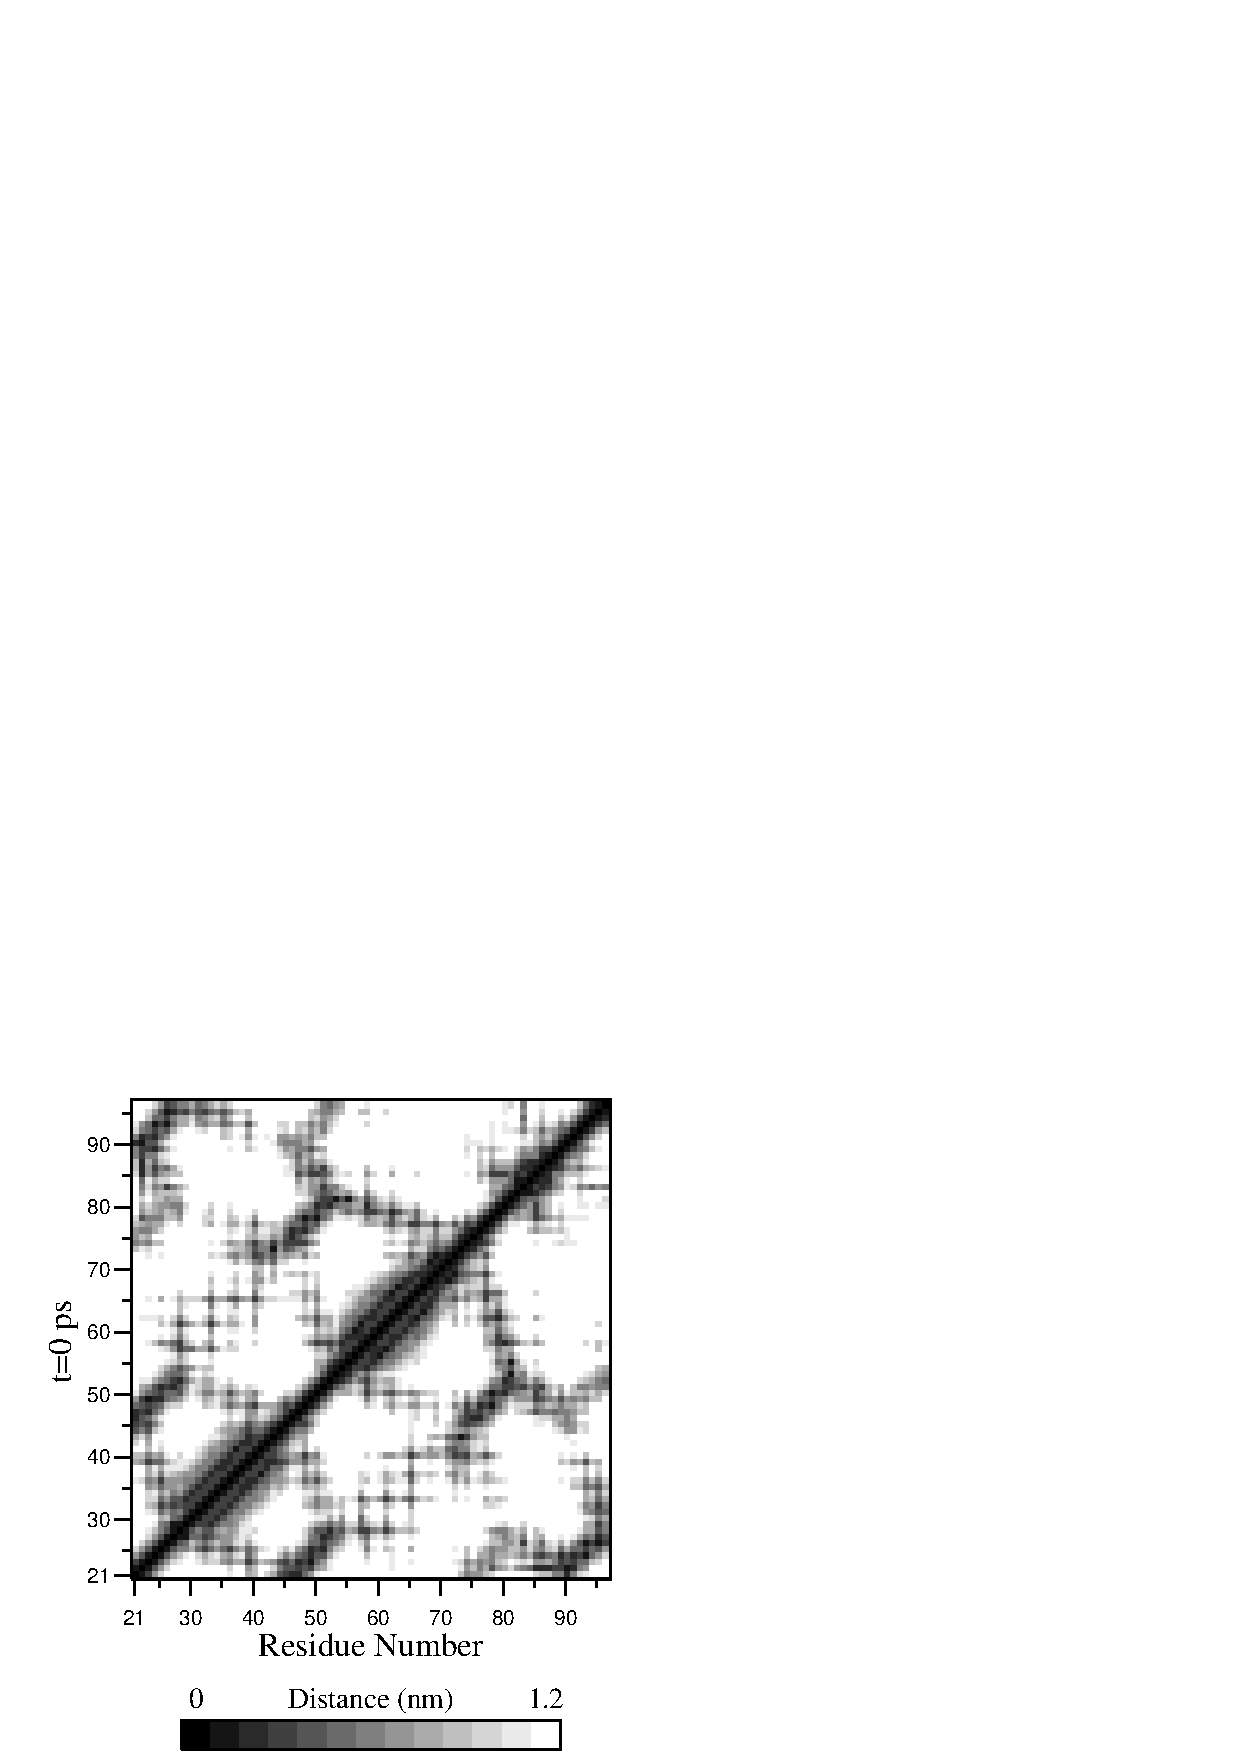
\includegraphics[width=6.5cm]{plots/distm}}
\caption{A minimum distance matrix for a peptide~\protect\cite{Spoel96b}.}
\label{fig:mdmat}
\end{figure}

Plotting these matrices for different time-frames, one can analyze changes 
in the structure, and {\eg} forming of salt bridges.
\end{description}

%%%%%%%%%%%%%%%%%%%%%%%%%%%%%%%%%%%%%%% Root mean square deviations 

\section{Root mean square deviations in structure}
\label{sec:rmsd}
{\tt g\_rms, g\_rmsdist}\\
The {\em root mean square deviation} ($RMSD$) of certain atoms in a molecule
with respect to a reference structure can be calculated with the program 
{\tt \normindex{g\_rms}} by least-square fitting the structure to the reference structure
($t_2 = 0$) and subsequently calculating the $RMSD$ (\eqnref{rmsd}).
\beq
RMSD(t_1,t_2) ~=~ \left[\frac{1}{M} \sum_{i=1}^N m_i \|{\bf r}_i(t_1)-{\bf r}_i(t_2)\|^2 \right]^{\frac{1}{2}}
\label{eqn:rmsd}
\eeq
where $M = \sum_{i=1}^N m_i$ and ${\bf r}_i(t)$ is the position of atom $i$ at time $t$.
{\bf NOTE} that fitting does not have to use the same atoms as the calculation
of the $RMSD$; {\eg}: a protein is usually fitted on the backbone atoms
(N,C$_{\alpha}$,C), but the $RMSD$ can be computed of the backbone
or of the whole protein.

Instead of comparing the structures to the initial structure at time $t=0$ 
(so for example a crystal structure), one can also calculate \eqnref{rmsd} 
with a structure at time $t_2=t_1-\tau$.
This gives some insight in the mobility as a function of $\tau$.
Also a matrix can be made with the $RMSD$ as a function of $t_1$ and $t_2$,
this gives a nice graphical impression of a trajectory.
If there are transitions in a trajectory, they will clearly show up in
such a matrix.

Alternatively the $RMSD$ can be computed using a fit-free method with the 
program {\tt \normindex{g\_rmsdist}}:
\beq
RMSD(t) ~=~     \left[\frac{1}{N^2}\sum_{i=1}^N \sum_{j=1}^N    \|{\bf r}_{ij}(t)-{\bf r}_{ij}(0)\|^2\right]^{\frac{1}{2}}
\label{eqn:rmsdff}
\eeq
where the {\em distance} {\bf r}$_{ij}$ between atoms at time $t$ 
is compared with the distance between the same atoms at time $0$.

\ifthenelse{\equal{\gmxlite}{1}}{}{
\section{\normindex{Covariance analysis}}
\label{sec:covanal}
Covariance analysis, also called
\seeindex{principal component analysis}{covariance analysis}
or \seeindex{essential dynamics}{covariance analysis}
\cite{Amadei93}{,} can find correlated motions.
It uses the covariance matrix $C$ of the atomic coordinates:
\beq
C_{ij} = \left \langle 
M_{ii}^{\frac{1}{2}} (x_i - \langle x_i \rangle)
M_{jj}^{\frac{1}{2}}  (x_j - \langle x_j \rangle)
\right \rangle
\eeq
where $M$ is a diagonal matrix containing the masses of the atoms
(mass-weighted analysis) or the unit matrix (non-mass weighted analysis).
$C$ is a symmetric $3N \times 3N$ matrix, which can be diagonalized with
an orthonormal transformation matrix $R$:
\beq
R^T C R = \mbox{diag}(\lambda_1,\lambda_2,\ldots,\lambda_{3N})
~~~~\mbox{where}~~\lambda_1 \geq \lambda_2 \geq \ldots \geq \lambda_{3N}
\eeq
The columns of $R$ are the eigenvectors, also called principal or
essential modes.
$R$ defines a transformation to a new coordinate system. The trajectory
can be projected on the principal modes to give the principal components
$p_i(t)$:
\beq
{\bf p}(t) = R^T M^{\frac{1}{2}} ({\bf x}(t) - \langle {\bf x} \rangle)
\eeq
The eigenvalue $\lambda_i$ is the mean square fluctuation of principal
component $i$. The first few principal modes often describe 
collective, global motions in the system.
The trajectory can be filtered along one (or more) principal modes.
For one principal mode $i$ this goes as follows:
\beq
{\bf x}^f(t) =
\langle {\bf x} \rangle + M^{-\frac{1}{2}} R_{*i} \, p_i(t)
\eeq

When the analysis is performed on a macromolecule, one often wants to
remove the overall rotation and translation to look at the internal motion
only. This can be achieved by least square fitting to a reference structure.
Care has to be taken that the reference structure is representative for the
ensemble, since the choice of reference structure influences the covariance
matrix.

One should always check if the principal modes are well defined.
If the first principal component resembles a half cosine and
the second resembles a full cosine, you might be filtering noise (see below).
A good way to check the relevance of the first few principal
modes is to calculate the overlap of the sampling between
the first and second half of the simulation.
Note that this can only be done when the same reference structure is
used for the two halves.

A good measure for the overlap has been defined in~\cite{Hess2002b}.
The elements of the covariance matrix are proportional to the square
of the displacement, so we need to take the square root of the matrix
to examine the extent of sampling. The square root can be
calculated from the eigenvalues $\lambda_i$ and the eigenvectors,
which are the columns of the rotation matrix $R$.
For a symmetric and diagonally-dominant matrix $A$ of size $3N \times 3N$
the square root can be calculated as:
\beq
A^\frac{1}{2} = 
R \, \mbox{diag}(\lambda_1^\frac{1}{2},\lambda_2^\frac{1}{2},\ldots,\lambda_{3N}^\frac{1}{2}) \, R^T
\eeq
It can be verified easily that the product of this matrix with itself gives
$A$.
Now we can define a difference $d$ between covariance matrices $A$ and $B$
as follows:
\begin{eqnarray}
d(A,B) & = & \sqrt{\mbox{tr}\left(\left(A^\frac{1}{2} - B^\frac{1}{2}\right)^2\right)
}
\\ & = &
\sqrt{\mbox{tr}\left(A + B - 2 A^\frac{1}{2} B^\frac{1}{2}\right)}
\\ & = &
\left( \sum_{i=1}^N \left( \lambda_i^A + \lambda_i^B \right)
- 2 \sum_{i=1}^N \sum_{j=1}^N \sqrt{\lambda_i^A \lambda_j^B}
\left(R_i^A \cdot R_j^B\right)^2 \right)^\frac{1}{2}
\end{eqnarray}
where tr is the trace of a matrix.
We can now define the overlap $s$ as:
\beq
s(A,B) = 1 - \frac{d(A,B)}{\sqrt{\mbox{tr}A + \mbox{tr} B}}
\eeq
The overlap is 1 if and only if matrices $A$ and $B$ are identical.
It is 0 when the sampled subspaces are completely orthogonal.

A commonly used measure is the subspace overlap of the first few
eigenvectors of covariance matrices.
The overlap of the subspace spanned by $m$ orthonormal vectors 
${\bf w}_1,\ldots,{\bf w}_m$ with a reference subspace spanned by 
$n$ orthonormal vectors ${\bf v}_1,\ldots,{\bf v}_n$
can be quantified as follows:
\beq
\mbox{overlap}({\bf v},{\bf w}) =
\frac{1}{n} \sum_{i=1}^n \sum_{j=1}^m ({\bf v}_i \cdot {\bf w}_j)^2
\eeq
The overlap will increase with increasing $m$ and will be 1 when
set ${\bf v}$ is a subspace of set ${\bf w}$.
The disadvantage of this method is that it does not take the eigenvalues
into account. All eigenvectors are weighted equally and when
degenerate subspaces are present (equal eigenvalues) the calculated overlap
will be too low.

Another useful check is the cosine content. It has been proven the
the principal components of random diffusion are cosines with the number of
periods equal to half the principal component index\cite{Hess2000,Hess2002b}.
The eigenvalues are proportional to the index to the power $-2$.
The cosine content is defined as:
\beq
\frac{2}{T}
\left( \int_0^T \cos\left(\frac{i \pi t}{T}\right) \, p_i(t) \mbox{d} t \right)^2
\left( \int_0^T p_i^2(t) \mbox{d} t \right)^{-1}
\eeq
When the cosine content of the first few principal components
is close to 1, the largest fluctuations are not connected with
the potential, but with random diffusion.

The covariance matrix is built and diagonalized by
{\tt \normindex{g\_covar}}.
The principal components and overlap (any many more things) 
can be plotted and analyzed with {\tt \normindex{g\_anaeig}}.
The cosine content can be calculated with {\tt \normindex{g\_analyze}}.
} % Brace matches ifthenelse test for gmxlite

\ifthenelse{\equal{\gmxlite}{1}}{}{
\section{Dihedral principal component analysis}
{\tt g\_angle, g\_covar, g\_anaeig}\\
Principal component analysis can be performed in dihedral
space~\cite{Mu2005a} using {\gromacs}. You start by defining the
dihedral angles of your interest in an index file, either using {\tt
  mk\_angndx} or otherwise. Then you use the {\tt g\_angle} program
with the -or flag to produce a new trr file containing the cosine and
sine of each dihedral angle in two coordinates respectively. That is,
in the trr file you will have a series of numbers corresponding to:
cos($\phi_1$), sin($\phi_1$), cos($\phi_2$), sin($\phi_2$), ...,
cos($\phi_n$), sin($\phi_n$), the array is padded with zeros if
necessary.  Then you can use this trr file as input for the {\tt
  g\_covar} program and perform principal component analysis as usual.
For this to work you will need to generate a reference file (tpr, gro,
pdb etc.) containing the same number of ``atoms'' as the new trr file,
that is for $n$ dihedrals you need 2$n$/3 atoms (rounded up if not an
integer number). You should use the {\tt -nofit} option for {\tt
  g\_covar} since the coordinates in the dummy reference file do not
correspond in any way to the information in the trr file. Analysis of
the results is done using {\tt g\_anaeig}.  }
 
%%%%%%%%%%%%%%%%%%%%%%%%%%%%%%%%%%%%%%% Hydrogen bonds

\section{Hydrogen bonds}
{\tt g\_hbond}\\
The program {\tt \normindex{g\_hbond}} analyses the {\em hydrogen bonds} (H-bonds)
between all possible donors D and acceptors A. To determine if an
H-bond exists, a geometrical criterion is used, see also
\figref{hbond}:
\beq
\begin{array}{rclcl}
r       & \leq  & r_{HB}        & = & 0.35 \mbox{nm}    \\
\alpha  & \leq  & \alpha_{HB}   & = & 30^o              \\
\end{array}
\eeq

\begin{figure}
\centerline{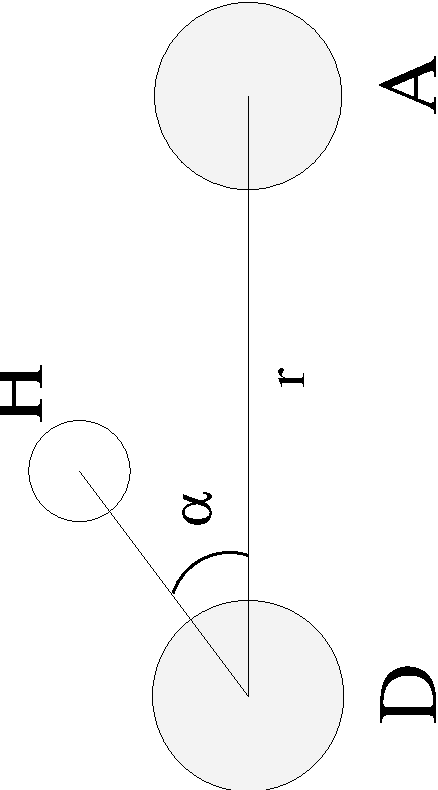
\includegraphics[width=2.5cm,angle=270]{plots/hbond}}
\caption{Geometrical Hydrogen bond criterion.}
\label{fig:hbond}
\end{figure}

The value of $r_{HB} = 0.35$~nm corresponds to the first minimum of the rdf of 
SPC-water (see also \figref{rdf}).

The program {\tt g\_hbond} analyses all hydrogen bonds existing
between two groups of atoms (which must be either identical or
non-overlapping) or in specified Donor Hydrogen Acceptor triplets, in
the following ways:

\begin{figure}
\centerline{
{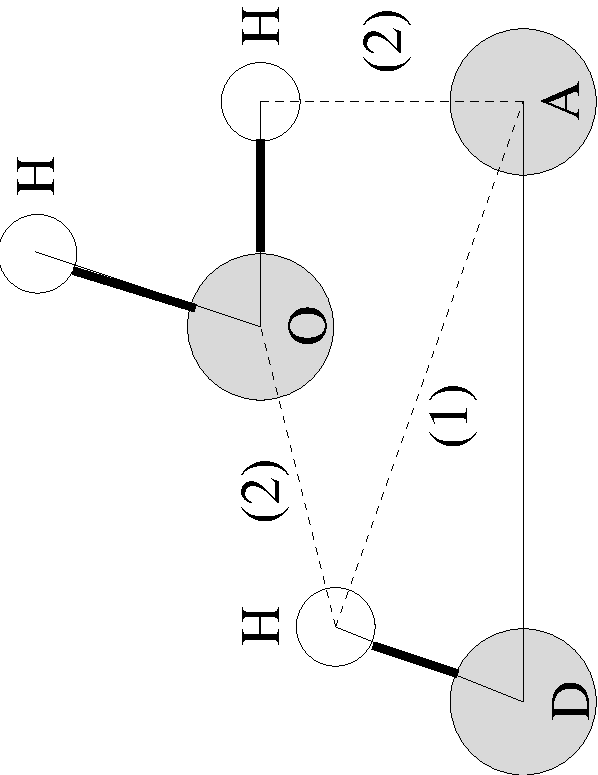
\includegraphics[width=5cm,angle=270]{plots/hbond_insert}}}
\caption[Insertion of water into an H-bond.]{Insertion of water into
an H-bond. (1) Normal H-bond between two residues. (2) H-bonding
bridge via a water molecule.}
\label{fig:insert}
\end{figure}

\begin{itemize}
\item
Donor-Acceptor distance ($r$) distribution of all H-bonds
\item
Hydrogen-Donor-Acceptor angle ($\alpha$) distribution of all H-bonds 
\item
The total number of H-bonds in each time frame
\item
\newcommand{\nn}[1]{$n$-$n$+$#1$}
The number of H-bonds in time between residues, divided into groups
\nn{i} where $n$ and $n$+$i$ stand for residue numbers and $i$ goes
from 0 to 6. The group for $i=6$ also includes all H-bonds for
$i>6$. These groups include the \nn{3}, \nn{4} and \nn{5} H-bonds
which provide a measure for the formation of $\alpha$-helices or
$\beta$-turns or strands.
\item
The lifetime of the H-bonds is calculated from the average over all
autocorrelation functions of the existence functions (either 0 or 1)
of all H-bonds:
\beq
C(\tau) ~=~ \langle s_i(t)~s_i (t + \tau) \rangle
\label{eqn:hbcorr}
\eeq
with $s_i(t) = \{0,1\}$ for H-bond $i$ at time $t$. The integral of
$C(\tau)$ gives a rough estimate of the average H-bond lifetime
$\tau_{HB}$:
\beq
\tau_{HB} ~=~ \int_{0}^{\infty} C(\tau) d\tau
\label{eqn:hblife}
\eeq
Both the integral and the complete auto correlation function $C(\tau)$
will be output, so that more sophisticated analysis ({\eg}\@ using
multi-exponential fits) can be used to get better estimates for
$\tau_{HB}$. A more complicate analysis is given in ref.~\cite{Spoel2006b},
one of the more fancy option is the Luzar and Chandler analysis
of hydrogen bond kinetics~\cite{Luzar96b,Luzar2000a}. 
\item
An H-bond existence map can be generated of dimensions {\em
\#~H-bonds}$\times${\em \#~frames}. The ordering is identical to the index 
file (see below), but reversed, meaning that the last triplet in the index
file corresponds to the first row of the existence map.
\item
Index groups are output containing the analyzed groups, all
donor-hydrogen atom pairs and acceptor atoms in these groups,
donor-hydrogen-acceptor triplets involved in hydrogen bonds between
the analyzed groups and all solvent atoms involved in insertion.
\item
Solvent insertion into H-bonds can be analyzed, see
\figref{insert}. In this case an additional group identifying
the solvent must be selected. The occurrence of insertion will be
indicated in the existence map. Note that insertion into and existence
of a specific H-bond can occur simultaneously and will also be
indicated as such in the existence map.
\end{itemize}

\ifthenelse{\equal{\gmxlite}{1}}{}{
%
%%%%%%%%%%%%%%%%%%%%%%%%%%%%%%%%%%%%%%% Protein related items 

\section{Protein related items}
{\tt do\_dssp, g\_rama, xrama, wheel}\\
To analyze structural changes of a protein, you can calculate the radius of 
gyration or the minimum residue distances during time 
(see \secref{rg}), or calculate the RMSD (\secref{rmsd}).

You can also look at the changing of {\em secondary structure elements} 
during your run. For this you can use the program {\tt \normindex{do\_dssp}}, which is 
an interface for the commercial program {\tt dssp}~\cite{Kabsch83}. For 
further information, see the {\tt dssp}-manual. A typical output plot of 
{\tt do\_dssp} is given in \figref{dssp}.

\begin{figure}
\centerline{
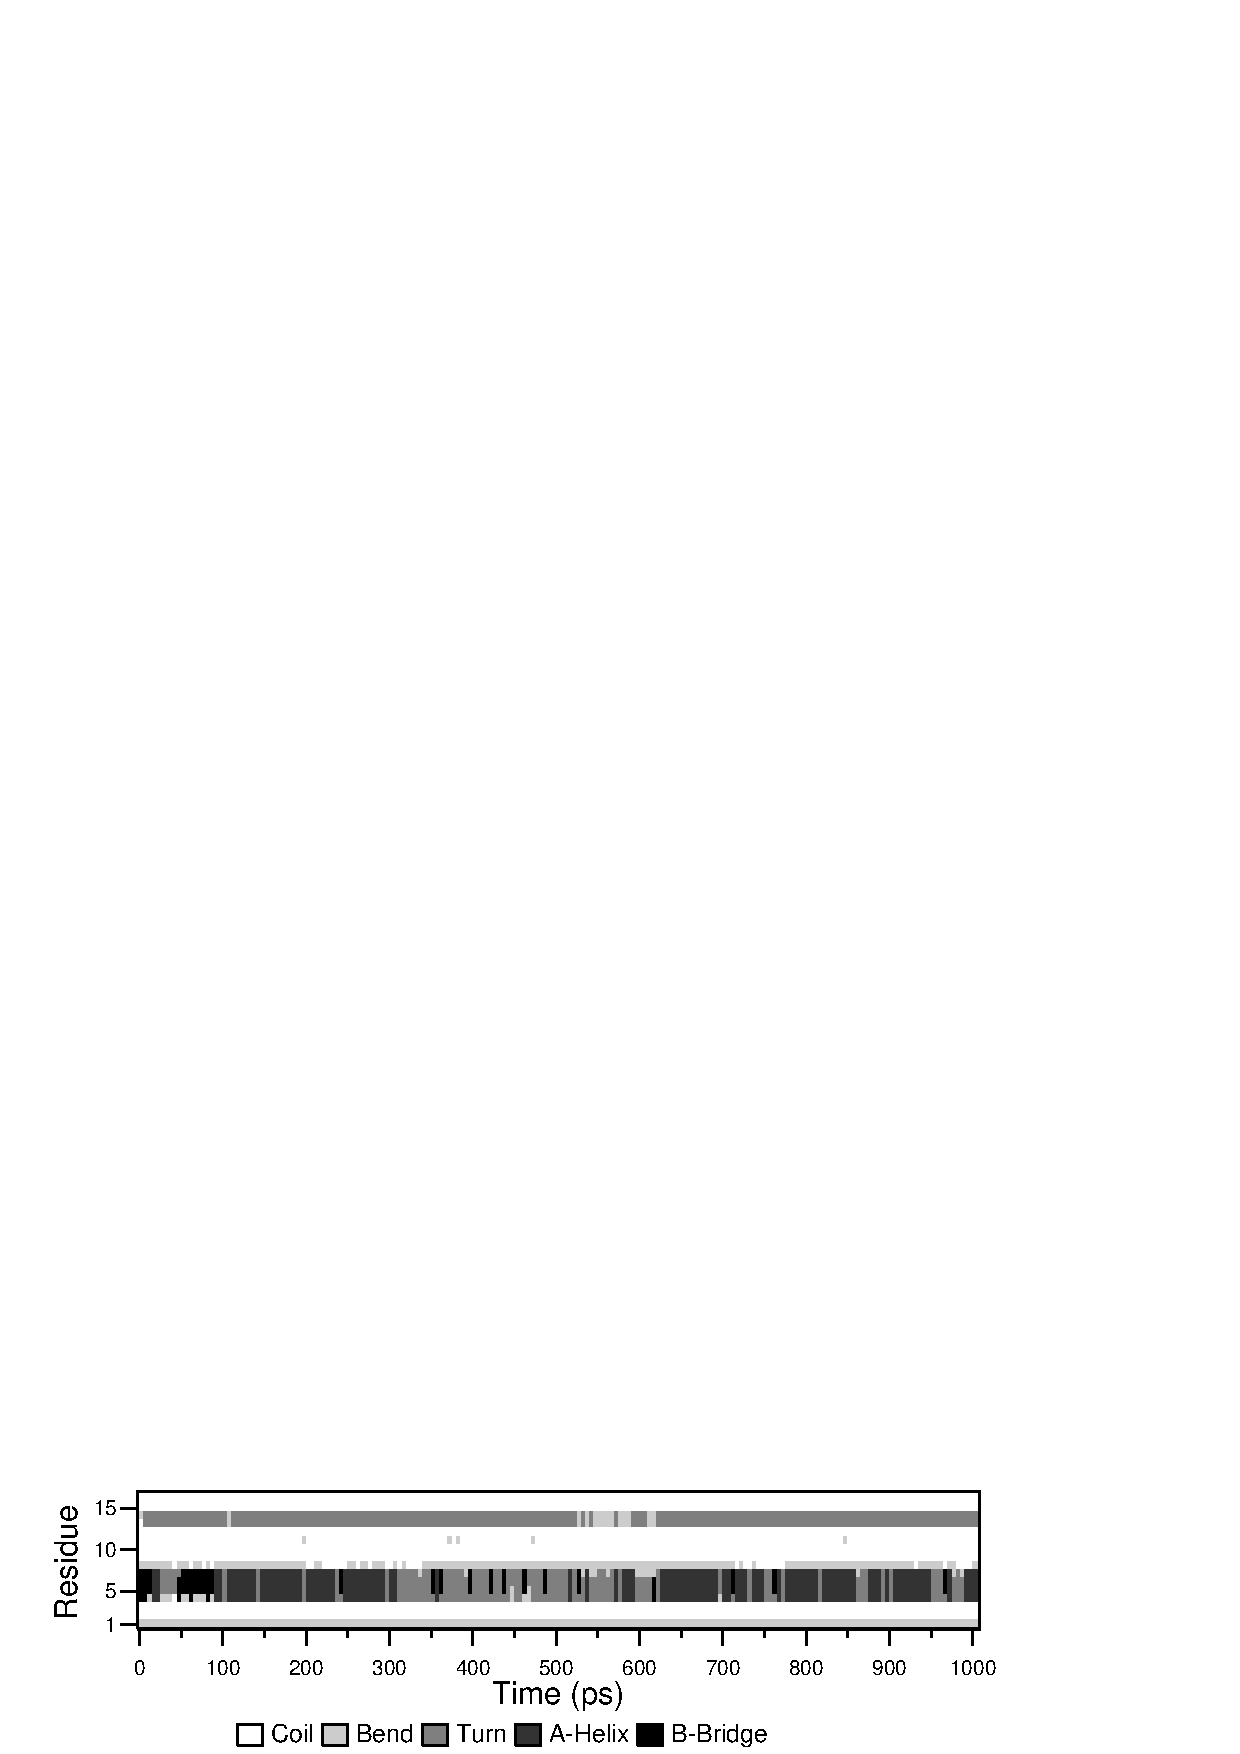
\includegraphics[width=12cm]{plots/dssp}}
\caption{Analysis of the secondary structure elements of a peptide in time.}
\label{fig:dssp}
\end{figure}

One other important analysis of proteins is the so called 
{\em Ramachandran plot}. 
This is the projection of the structure on the two dihedral angles $\phi$ and 
$\psi$ of the protein backbone, see \figref{phipsi}.

\begin{figure}
\centerline{
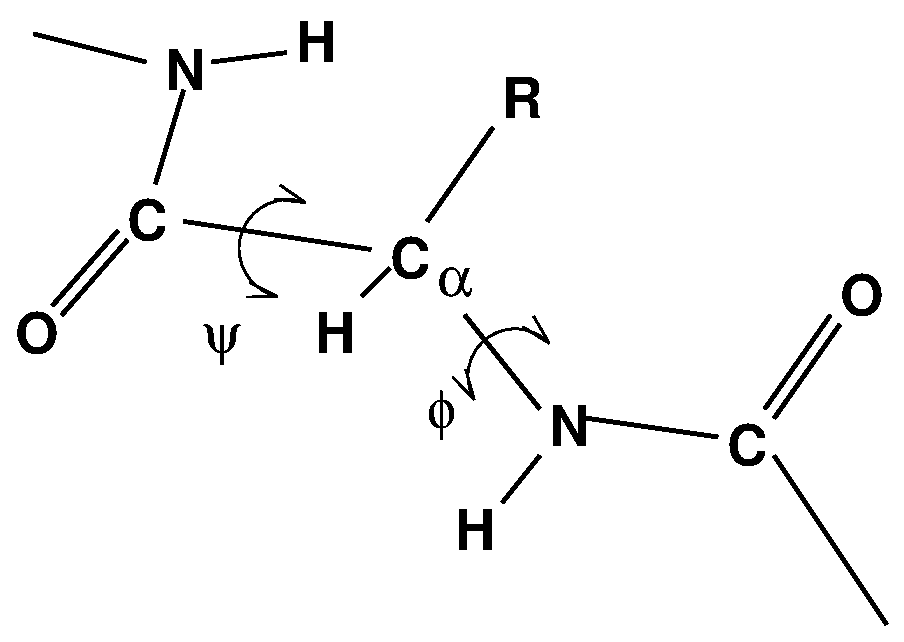
\includegraphics[width=5cm]{plots/phipsi}}
\caption{Definition of the dihedral angles $\phi$ and $\psi$ of the protein backbone.}
\label{fig:phipsi}
\end{figure}

To evaluate this Ramachandran plot you can use the program {\tt \normindex{g\_rama}}. 
A typical output is given in \figref{rama}.

\begin{figure}
\centerline{
{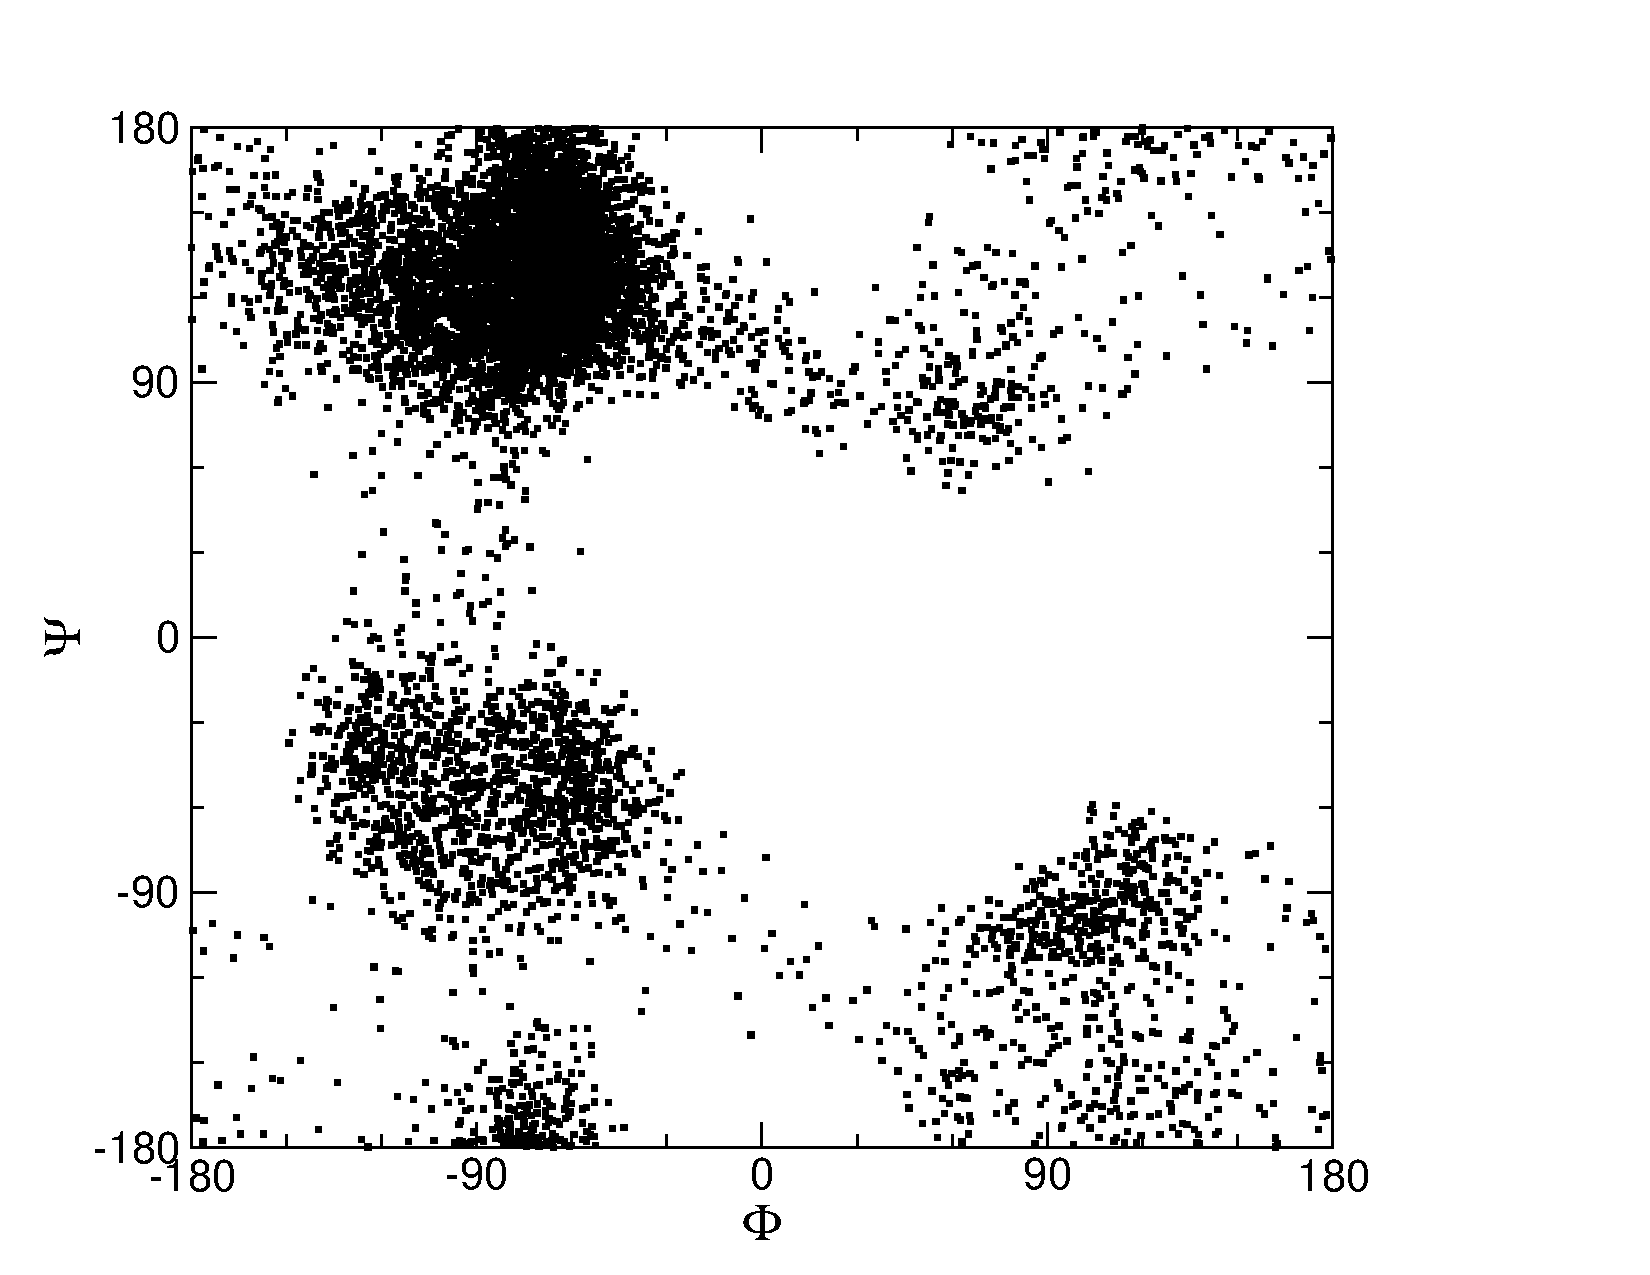
\includegraphics[width=8cm]{plots/rama}}}
\caption{Ramachandran plot of a small protein.}
\label{fig:rama}
\end{figure}

It is also possible to generate an animation of the Ramachandran plot
in time. This can be of help for analyzing certain dihedral transitions 
in your protein. You can use the program {\tt \normindex{xrama}} for this.

When studying $\alpha$-helices 
it is useful to have a {\em helical wheel} projection
of your peptide, to see whether a peptide is amphipatic. This can be done
using the {\tt \normindex{wheel}} program. Two examples are 
plotted in \figref{wheel}.

\begin{figure}
\centerline{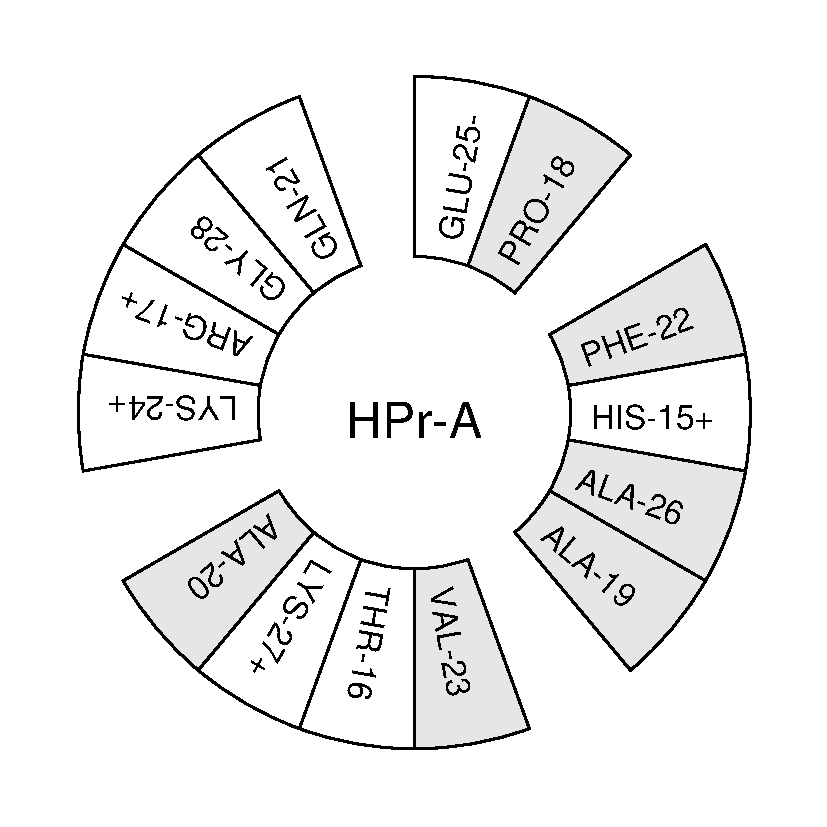
\includegraphics[width=\htw]{plots/hpr-wheel}}
\caption{Helical wheel projection of the N-terminal helix of HPr.}
\label{fig:wheel}
\end{figure}

%%%%%%%%%%%%%%%%%%%%%%%%%%%%%%%%%%%%%%% Membrane Related Items

\section{Interface related items}
{\tt g\_order, g\_density, g\_potential, g\_traj}\\
When simulating molecules with long carbon tails, it can be
interesting to calculate their average orientation. There are several
flavors of order parameters, most of which are related. The program
{\tt \normindex{g\_order}} can calculate order parameters using the equation

\begin{equation}
S_{z} = \frac{3}{2}\langle {\cos^2{\theta_z}} \rangle - \frac{1}{2}
\label{eqn:Sgr}
\end{equation}
where $\theta_z$ is the angle between the $z$-axis of the simulation
box and the molecular axis under consideration. The latter is defined as the
vector from C$_{n-1}$ to C$_{n+1}$. The parameters $S_x$
and $S_y$ are defined in the same way. The brackets imply averaging over time
and molecules. Order parameters can vary between 1 (full order along
the interface normal) and $-1/2$ (full order perpendicular to the
normal), with a value of zero in the case of isotropic orientation.

The program can do two things for you. It can calculate the order
parameter for each CH$_2$ segment separately, for any of three axes,
or it can divide the box in slices and calculate the average value of
the order parameter per segment in one slice. The first method gives
an idea of the ordering of a molecule from head to tail, the second
method gives an idea of the ordering as function of the box length.

The electrostatic potential ($\psi$) across the interface can be
computed from a trajectory by evaluating the double integral of the
charge density ($\rho(z)$):
\beq
\psi(z) - \psi(-\infty) = - \int_{-\infty}^z dz' \int_{-\infty}^{z'} \rho(z'')dz''/ \epsilon_0 
\label{eqn:elpotgr}
\eeq
where the position $z=-\infty$ is far enough in the bulk phase that
the field is zero.  With this method, it is possible to ``split'' the
total potential into separate contributions from lipid and water
molecules. The program {\tt \normindex{g\_potential}} divides the box in slices and
sums all charges of the atoms in each slice. It then integrates this
charge density, giving the electric field, and the electric field,
giving the potential. Charge density, field and potential are written
to {\tt xvgr-}input files.

The program {\tt \normindex{g\_traj}} is a very simple analysis program. All it
does is print the coordinates, velocities or forces of selected atoms.
It can also calculate the center of mass of one or more
molecules and print the coordinates of the center of mass to three
files. By itself, this is probably not a very useful analysis, but
having the coordinates of selected molecules or atoms can be very
handy for further analysis, not only in interface systems.

The program {\tt \normindex{g\_pvd}} calculates a lot of properties, among which
the density of a group in particles per unit of volume, but not a
density that takes the mass of the atoms into account. The program
{\tt \normindex{g\_density}} also calculates the density of a group, but takes the
masses into account and gives a plot of the density against a box
axis. This is useful for looking at the distribution of groups or
atoms across the interface.

%%%%%%%%%%%%%%%%%%%%%%%%%%%%%%%%%%%%%%% Chemical shifts

\section{Chemical shifts}
{\tt total, do\_shift}\\
You can compute the NMR chemical shifts of protons with the program
{\tt \normindex{do\_shift}}. This is just an {\gromacs} interface to
the public domain program {\tt total}~\cite{Williamson93a}. For
further information, read the article. Although there is limited
support for this in {\gromacs} users are encouraged to use the
software provided by the David Case group at Scripps because it seems
to be more up-to-date.

%%%%%%%%%%%%%%%%%%%%%%%%%%%%%%%%%%%%%%%
} % Brace matches ifthenelse test for gmxlite
